%! TeX root = ../charles/en/thesis.tex
\chapter{Results}
\label{chap:results}

In this chapter we evaluate the performance of post-pretraining the Merlot
Reserve model on our proposed dataset from \cref{chap:setup}. We test
downstream performance on STAR~\citep{wu2021star} and
NExT-QA~\citep{xiao2021nextqa}, and analyse some of the choices we made in our
dataset design process. We finish with a comparison
to~\citep{bagad2023testoftime}.

\section{Zero-Shot Downstream Results}
\label{sec:zs_results}

\subsection{STAR Results}
\label{ssec:star_results}

We report zero-shot performance of our model compared to the original Merlot Reserve
model in \cref{tab:star_ppt}. We find that performance improves slightly for both
validation and test splits. We especially observe a noticeable gain in performance
on prediction questions. These have a temporal element to them, although we do not
target this kind of hypothetical question type in our post-pretraining.

\begin{table}[t]
	\centering
	\caption{Zero-shot STAR accuracy on Merlot Reserve and our post-pretrained
	model. Our model improves on Merlot Reserve for all question types.}
	\label{tab:star_ppt}
	\begin{tabular}{lccccc}
        \toprule
        \multicolumn{1}{c}{}        & \multicolumn{4}{c}{Question Types}        & \multicolumn{1}{c}{} \\
                                      \cmidrule(){2-5}
                                    & I           & S        & P          & F           & Mean \\
        \cmidrule(r){1-1}             \cmidrule(){2-5}                          \cmidrule(l){6-6}
    Merlot Reserve (val)        & 43.12       & 42.33    & 43.27      & 47.14       & 43.01\\
%	Swapped before/after		&			  & 42.92    &			  &				& \\
%	Masked temporal expressions &			  & 50.86    &			  &				& \\
%	Shuffled frames				& 42.08		  & 42.58	 & 47.28	  & 49.20		& 38.47 \\
%    \cmidrule(r){1-1}             \cmidrule(){2-5}                          \cmidrule(l){6-6}
%	5500 steps					& 35.86		  & 40.43	 & 46.79	  & 45.10		& 39.77 \\
%	Swapped before/after		&			  & 39.88	 &			  &				& \\
%	Masked temporal expressions &			  & 43.08    &			  &				& \\
%	Shuffled frames				& 36.27		  & 37.90	 & 51.52	  & 39.39		& 38.47 \\
%    \cmidrule(r){1-1}             \cmidrule(){2-5}                          \cmidrule(l){6-6}
%	19500 steps					& 39.16		  & 41.83    & 48.55	  & 45.31		& 41.76 \\
%	Swapped before/after		&			  & 41.27	 &			  &				& \\
%	Masked temporal expressions &			  & 42.30    &			  &				& \\
%	Shuffled frames				& 39.32		  & 42.30	 & 52.72	  & 49.18		& 42.68 \\
%    \cmidrule(r){1-1}             \cmidrule(){2-5}                          \cmidrule(l){6-6}
%	22500 steps					& 40.95		  & 43.20    & 50.32	  & 48.16		& 43.41 \\
%	Swapped before/after		& 			  &	42.89    &			  &				& \\
%	Masked temporal expressions &			  & 43.08    &			  &				& \\
%	Shuffled frames				& 41.83		  & 43.53	 & 52.88	  & 52.24		& 44.38 \\
%	\midrule
%	\midrule
%	\multicolumn{6}{c}{Performance degrades with masking only temporal expressions} \\
%	20000 steps					& 30.82		  &	35.02	 & 38.14	  &	37.76		& 34.07 \\
%	Swapped before/after		&			  &	34.69	 &			  &				& \\
%	Masked temporal expressions	&			  &			 &			  &				& \\
%	Shuffled frames				&   &  &   &  & \\
%    \cmidrule(r){1-1}             \cmidrule(){2-5}                          \cmidrule(l){6-6}
%	41000 steps					& 30.86		  & 34.69    & 37.82      & 38.57       & 33.94 \\
%	Swapped before/after		&			  & 34.33	 &		      &				& \\
%	Masked temporal expressions &			  & 43.20	 &			  &				& \\
%	Shuffled frames				& 31.15		  & 34.41	 & 37.18	  & 38.16		& 33.81 \\
%	\midrule
%	\midrule
%	\multicolumn{6}{c}{Mixed temporal sparse} \\
%	25000 steps					& 38.99 & 40.3 & 48.2 & 51.2 & 41.3 \\
%	Swapped before/after		&		& 39.65 &	&		& \\
%	Shuffled frames				& 38.41 & 40.52 & 49.2 & 50.2 & 41.2 \\
%	\midrule
%	\midrule
%		\multicolumn{6}{c}{Updated charades\_parser} \\
		%Ours (13500 steps)			& 39.41 & 39.79 & 47.76 & 46.94 & 40.86 \\
		%Swapped before/after		&		& 40.83	&		&		&	\\
		%Shuffled frames				&  &  &  &  &  \\
%		\midrule
		%Ours (22500 steps)			& 39.12 & 40.18 & 48.88 & 48.16 & 41.14 \\
%		Swapped before/after		&		&  &		&		&	\\
%		Shuffled frames				&  &  &  &  &  \\
		Ours (val)			& 43.99 & 43.64 & 50.48 & 47.96 & 44.66 \\
		\midrule
		Merlot Reserve (test) & 40.51 & 44.76 & 43.85 & 39.48 & 42.15 \\
		Ours (test)			& 41.49 & 44.88 & 46.09 & 40.70 & 43.29 \\
        \bottomrule
%		Interaction Accuracy: 0.39115929941618016
%Sequence Accuracy: 0.401840490797546
%Prediction Accuracy: 0.48878205128205127
%Feasibility Accuracy: 0.4816326530612245
%Overall Accuracy: 0.41138348830656524
	\end{tabular}
\end{table}


We go back to the probing experiments from \cref{chap:probe}, and ask how our
model performs under the same conditions. Results are shown in
\cref{tab:probe_final}. There is little change except in the masked temporal
expressions task, which shows weaker performance in our trained model.
Surprisingly, despite our dataset having an even split of inverse relations, we
note a strong bias towards answering ``before'' for this masked temporal
expressions task, and would be worthy of future investigation. We also note
that in some other models we tested there would be a strong bias towards
``after''.

\begin{table}[t]
	\centering
	\caption{Probing Sequence Questions on validation data. Comparisons in
	brackets are compared to validation sequence values in \cref{tab:star_ppt}.
	For swap and shuffle frames, a lower change is better.}
	\label{tab:probe_final}
	\begin{tabular}{lccc}
	\toprule
	Model & Swap ($+/-\downarrow$) & Shuffle Frames ($+/-\downarrow$) & Mask ($\uparrow$) \\
	\cmidrule(r){1-1}             \cmidrule(){2-3} \cmidrule(l){4-4}
	Chance			& \multicolumn{2}{c}{25.00} & 50.00 \\
        \cmidrule(r){1-1}             \cmidrule(){2-3} \cmidrule(l){4-4}
		Merlot Reserve & 42.92 (+0.59) & 42.58 (\textbf{+0.25})  & \textbf{50.86} \\
%		VideoCLIP & & & \\
%		Ours & 40.66 (+0.48) & 40.88 (+0.70) & 56.97 \\
		Ours & 43.98 (\textbf{+0.34}) & 44.67 (+1.03) & 44.81 \\
	\bottomrule
	\end{tabular}
\end{table}

\subsection{NExT-QA Results}
\label{sec:nextqa_results}
%NExT-QA results (\cref{tab:nextqa}). Questions are interesting, generally a bit of a drop, but huge loss in performance for counting questions.

To test the generalisability of our approach to a wider range of temporal
relations, and a different domain, we also test zero-shot on NExT-QA. As in
\cref{sec:mres_zs}, we convert NExT-QA questions into statements to minimise
distribution drift. Since each question is hand-written and does not follow a
strict template for question types, we use a generative \acrshort{llm} to
convert from questions to masked statements. We follow the approach in
\citet{zellers2022mreserve} for generating statements for
MSRVTT-QA~\citep{xu2016msr-vtt} questions, by providing a prompt for each
question type. We use Mistral-7B-Instruct~\citep{jiang2023mistral}, an
\acrshort{llm} which has been finetuned to better respond to instructional
prompts (see~\citet{ouyang2022instructgpt}). For each question, we provide a
different prompt depending on the question type, which includes an instruction
of the task, three examples taken from the training set with hand-written
statement conversions, and finally the question which is to be converted. An
example for Temporal Next (TN) questions, asking what will happen after an
event, is shown below:

\begin{verbatim}
system: "You are a helpful assistant. The user will give an input
        question, and you will respond with the question in the
        form of a statement, giving space for an answer in the
        form of an underscore."
user: "what does the girl do after placing the mop down"
assistant: "the girl _ after placing the mop down"
user: "how does the child react after falling over"
assistant: "the child _ after falling over"
user: "what did the boy do after he stopped playing the drums the 
      second time"
assistant: "the boy _ after he stopped playing the drums the 
           second time"
user: ${question}
assistant: 
\end{verbatim}

We confirm that the output is valid by checking that there is one mask token
per generated statement, and manually editing if there was not. We found 25
examples that had to be manually edited, predominantly for questions such as
asking to describe the colour of clothes worn by multiple people, where the
answer is actually the same for both people.

We show our results in \cref{tab:nextqa}. We compare the performance on Merlot
Reserve using our generated statements with using the existing questions and
adding a mask token at the end of the question, simulating where an answer to
the question would ordinarily go, and observe overall better performance using
statements (35.0 vs 32.2), confirming that the generation process helps to
mitigate distribution shift. We then evaluate our post-pretrained model on the
ATP\textsubscript{hard} subset. Similarly to STAR, we find that main task
performance improves with our new model, although on the shuffled frames probe
we find that the model is not robust to the perturbation, with even improved
performance across most question types.

\begin{table}[t]
	\centering
	\caption{NExT-QA Results on Merlot Reserve. On the ATP\textsubscript{hard}
		subset, our model improves over Merlot Reserve, but neither model is
		robust at rejecting shuffled video features.  Column headings are:
		Causal How, Causal Why,
	Temporal Current, Temporal Next, Temporal Previous, Descriptive Location,
	Descriptive Count, Descriptive Other.}
	\label{tab:nextqa}
	\begin{tabular}{lccccccccc}
		\toprule
		\multicolumn{1}{c}{}  & \multicolumn{8}{c}{Question Types} & \multicolumn{1}{c}{}   \\
                                      \cmidrule(){2-9}
		Method			      &  CH  &  CW  &  TC  &  TN  &  TP  &  DL  &  DC  &  DO  & Mean \\
		\cmidrule(r){1-1}             \cmidrule(){2-10}
		Chance				  & \multicolumn{9}{c}{20.0} \\
		\cmidrule(r){1-1}             \cmidrule(){2-10}
		MReserve (val)        & 33.2 & 36.7 & 27.8 & 35.6 & 40.7 & 35.0 & 41.0 & 42.6 & 35.0 \\
		With Questions		  & 35.3 & 34.0 & 29.8 & 31.4 & 30.8 & 15.8 & 34.8 & 25.9 & 32.2 \\
%		Shuffled Frames		  & 33.5 & 35.7 & 28.9 & 36.0 & 36.9 & 35.0 & 40.0 & 38.9 & 34.6 \\
		\midrule
		\midrule
		%\cmidrule(r){1-1}             \cmidrule(){2-10}
		ATP\textsubscript{hard}	&28.9 & 27.5 & 29.8 & 25.8 &17.2 &  	&      &      & 27.5 \\
		Shuffled Frames		  & 29.7 & 27.7 & 30.0 & 24.7 & 24.1 &      &      &      & 27.6 \\
		\cmidrule(r){1-1}             \cmidrule(){2-10}
		%Ours ATP			  &	23.2 & 25.8 & 26.4 & 21.7 &	10.3 &  	&      &      & 24.3 \\
		%Shuffled Frames		  & 23.2 & 26.2 & 27.0 & 20.6 & 10.3 &      &      &      & 24.3 \\
		%Ours ATP			  & 23.7 & 28.4 & 30.3 & 21.7 & 24.1 &		&		&	  & 26.3 \\
		%Shuffled Frames		  & 25.0 & 29.4 & 30.3 & 21.9 & 17.2 &		&		&	  & 26.8 \\
		% \midrule
		Ours ATP			  & 27.9 & 29.1 & 32.5 & 27.1 & 27.6 & & & & 29.0 \\
		Shuffled Frames		  &	26.3 & 30.4	& 33.6 & 28.2 &	31.0 & & & & 29.7 \\
		\bottomrule
	\end{tabular}
\end{table}



\section{Qualitative Examples}
\label{sec:qualresults}

%Show some examples of predictions we get right, Merlot Reserve gets wrong,
%(and reverse?).
%We look at qualitative outputs. Compare examples which each version gets wrong.
%Generalisability of the approach with NExT-QA.

\Cref{fig:qual_example} shows an example where the post-pretrained model is
able to reason more about before and after than the original Merlot Reserve
model. Both Models get the original question right, but when we swap the
temporal relation in the statement, our model becomes a lot more uncertain and
selects a different answer, ``happy''. Note there is no ground truth for the
swapped statement. From the provided frames, it is quite possible that neither
predicted answer is correct for the swapped statement. Using open-ended
question answering may provide more insight into how a model approaches a task
with incorrect data.

\begin{figure}[t]
	\centering
	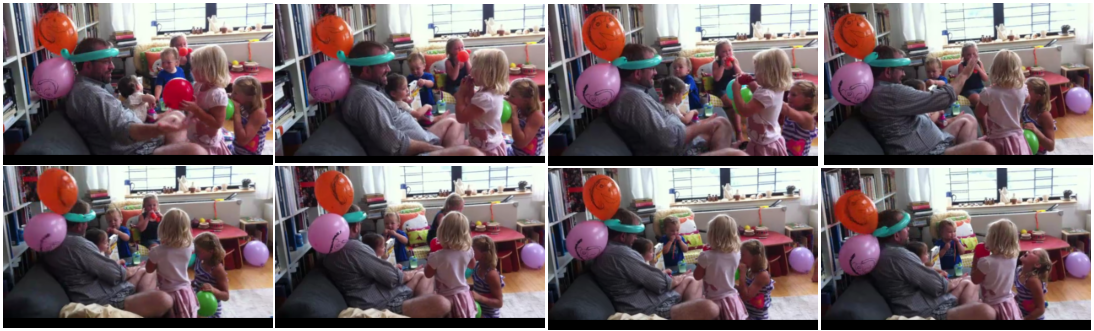
\includegraphics[width=1\textwidth]{qual_example}
	\caption{NExT-QA zero-shot example. Frames are ordered top row, then bottom row.
		Statement: \textsc{the girl in black was \_ before she stood up near the end}\\
		Swapped: \textsc{the girl in black was \_ after she stood up near the end}\\
		Our model predicts the correct answer,
		``blowing''  when presented with the correct statement, and predicts a
		different answer, ``happy'',  when the statement is swapped. Merlot
	Reserve predicts ``blowing'' for both statements.}
	\label{fig:qual_example}
\end{figure}

We also observe that the model can be limited in its ability to predict the
correct answer just based on the frames selected. \Cref{fig:frame_issue} shows
an example where the correct answer, ``raised his hand to the camera'' is not
shown in any of the frames provided to the model, and so it is very hard for
the model to select the correct answer from its inputs. A simple solution is to
provide more frames as input, use ensembles of models with different frame
selection processes, or use selection methods such
as~\citet{buch2022revisiting, lei2023revealing} for selecting informative
frames from a video.

\begin{figure}[t]
	\centering
	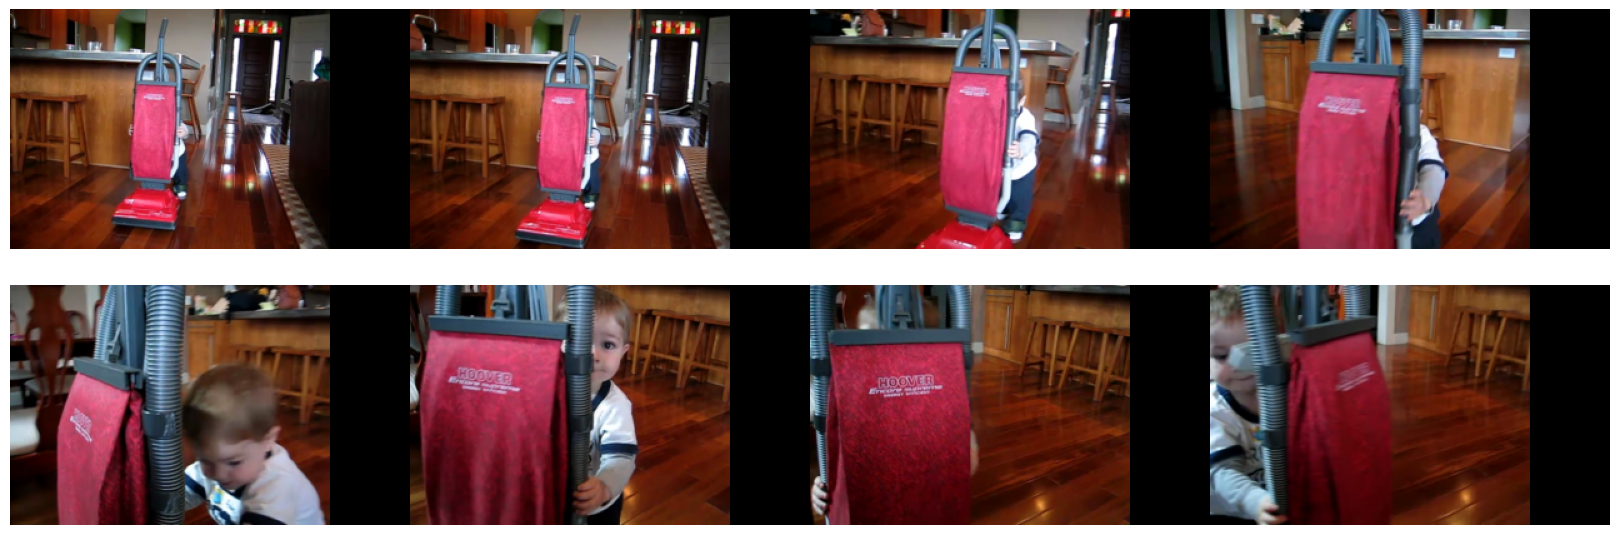
\includegraphics[width=\textwidth]{frame_issue}
	\caption{Frame selection means the model can have very little chance of selecting
	the correct answer.\\
	Statement: \textsc{the baby \_ after he approached near the camera}\\
	Prediction is ``suck his thumb'', ground truth is ``raised his hand to the camera''}
	\label{fig:frame_issue}
\end{figure}

\section{Expanding Temporal Relation Types}
\label{sec:expandtemprel}

We look at the effect of training with only inverse relation types as negative
span candidates, as opposed to a range of negatives to provide a more
fine-grained temporal understanding. We find that using more relation types
improves performance on sequence questions, with an accuracy of 43.64 compared
to 40.18 using only inverse relations.

%\begin{table}[t]
%	\centering
%	\caption{Comparison of number of temporal relations used (Val data).
%	}
%	\label{tab:expandtemprel}
%	\begin{tabular}{lcc}
%		\toprule
%		& STAR (Sequence) \\
%		\midrule
%		Non-overlapping & 40.18 \\
%		All relation types & 43.64 \\
%		\bottomrule
%	\end{tabular}
%\end{table}


\section{Selecting Annotation Method}
\label{sec:annot_method}

We also explore alternative approaches for creating the segments. Remember from
\cref{ssec:create_segs} that we split labels across three segments, combining
action annotations across segment boundaries depending on relation type. We
experiment with creating segments formed distinctly of the action annotation
and temporal expression in different segments, i.e. \mbox{[X;$\tau$;Y]} for
actions $X$, $Y$, and temporal relation type $\tau$. We find that this
significantly degrades performance (\cref{tab:annot_method}), and hypothesise
that this is due to the shorter length of the temporal relation, often just a
single token, which differs significantly from the length of segments found in
pre-training.

\begin{table}[t]
	\centering
	\caption{Annotation Method results on STAR (validation set). We test with
	spans that contain only temporal words compared to including part of action
	annotations in the masked temporal span.}
	\label{tab:annot_method}
	\begin{tabular}{lcc}
		\toprule
		 & Sequence & Mean (All) \\
		\midrule
		Combination & 43.64 & 44.66 \\
		Only temporal & 34.69 & 33.94 \\
		\bottomrule
	\end{tabular}
\end{table}


%TODO: explain this better
%We further explore using more dense annotations, with multiple relations per
%instance. We attempt to include as many relations as possible, with the
%requirement that relations cannot overlap with one another in time.  Where
%there is an overlap, there is a precedence order of relations: \textit{meets}
%\textgreater~\textit{overlaps} \textgreater~\textit{starts}
%\textgreater~\textit{finishes} \textgreater~\textit{during}
%\textgreater~\textit{equals} \textgreater~\textit{precedes}. This ordering
%prioritises relations that occur closer together, allowing for more relations
%in a single instance.
%
%Frames are selected based on $(X_{start}, X_{end}), (Y_{start}, Y_{end})$ and
%the specific relation type. If a relation requires frames that intersect an
%already selected frame, the relation is discarded. This is to keep a strict
%relationship between actions and time relations. Once all relations have been
%processed, any remaining frames up to 8 (the number of frames used in Merlot
%Reserve) are selected uniformly at the beginning or end, depending on the time
%before and after any relations. %Maybe more detail on exactly what is done here?
%
%Each frame associated with a relation is annotated with the associated actions
%$X$ and $Y$, along with a temporal indicator based on the specific relation
%type.
%
%For example, for a 30 second video, one relation may select two frames
%at 11 and 17 seconds, based on the times of the relation's actions. If a second
%relation requires frames at 15 and 19 seconds, this relation would be scrapped,
%since the alignment of the text description to their respective frames becomes
%impossible.

%\section{Freezing Layers}
%
%We test freezing different layers of the model, and find little difference
%TODO: table for these results


\section{Comparison to Test of Time}
\label{sec:tactcompare}

Finally, we compare our results to Test of Time~\citep{bagad2023testoftime}. We
run their TACT model, trained on TEMPO, on our perturbation tests
from~\cref{chap:probe}~(\cref{tab:tot_star}). We find that TACT performs
slightly worse than VideoCLIP  overall, although the probes achieve a
greater loss, suggesting that the model has increased uncertainty for those
tricky cases. Note the sequence column, which sees a drop of just under 1\%
on the base VideoCLIP model, but over 2\% when post-pretrained with TACT, on
the swapped before/after test.


As~\citet{bagad2023testoftime} mention, their approach was most successful on
VideoCLIP. On other models (Frozen~\citep{bain2021frozen},
VindLU~\citep{cheng2023vindlu}, CLIP4CLIP~\citep{luo2022clip4clip}), their
performance is not as strong. They hypothesise that this is due to the number
of frames provided as input to the model, with 32 provided to VideoCLIP
compared to a maximum of 12 in others. Merlot Reserve only provides 8, and as
our findings in~\cref{sec:qualresults} suggest, this may be a limiting factor
on further improving performance in this direction.

In comparison to Test of Time, we develop a dataset that trains on full videos,
rather than stitched together clips. This allows us to use a wider range of
temporal relations, based on Allen's Interval Algebra, that results in improved
downstream performance on sequence questions~(\cref{sec:expandtemprel}).
%See \cref{tab:tot_star}. Different base model. They use VideoCLIP~\citep{xu2021videoclip}, which performs well,
%but other models do not perform so well, e.g. Frozen~\citep{bain2021frozen}, 
%VindLU~\citep{cheng2023vindlu}, CLIP4CLIP~\citep{luo2022clip4clip}. They hypothesise
%that it may be because of number of frames input to the model. We use Merlot Reserve,
%which has 8 frames compared to VideoCLIP's 32. Poor results on this would indicate
%more frames is better for this task.

%Real-world data. We use full clips rather than stitched together. We use wider range
%of temporal relations (not just before/after).

\begin{table}[tp] 
    \centering 
    \caption{Test of Time (TEMPO TACT) accuracy on STAR validation set. Overall performance is
	lower than the base model VideoCLIP, but there is a slightly wider performance gap
	in the perturbations.}
    \label{tab:tot_star} 
    \begin{tabular}{lccccc} 
        \toprule
        \multicolumn{1}{c}{}    & \multicolumn{4}{c}{Question Types}            & \multicolumn{1}{c}{} \\
                                    \cmidrule(){2-5}
                                & I           & S        & P          & F           & Mean \\
        \cmidrule(r){1-1}           \cmidrule(){2-5}                                    \cmidrule(l){6-6}
        VideoCLIP		        & 39.66       & 42.86    & 48.72      & 50.82       & 42.84 \\
		Swapped before/after	&			  & 41.91	 &			  &				& \\
		Masked temporal expressions   &			  & 50.11    &			  &				& \\
		Shuffled videos			& 34.61		  & 36.31	 & 36.70	  & 40.82		& 36.08 \\
		Shuffled frames			& 39.99		  & 43.06	 & 46.47	  & 49.59		& 43.39 \\
		\midrule
		TEMPO TACT				& 39.49		  & 39.88	 & 47.44	  & 46.33		& 40.86 \\
		Swapped before/after    &			  & 37.73    &			  &				& \\
		Masked temporal expressions   &			  & 57.53    &			  &				& \\
		Shuffled videos			& 34.15		  & 33.27	 & 39.26	  & 37.14		& 34.36 \\
		Shuffled frames			& 38.49		  & 38.09	 & 44.55	  & 42.25		& 39.08 \\
        \bottomrule
    \end{tabular} 
\end{table} 

\section{Summary}
\label{sec:res_summary}

We have looked at the performance of our proposed post-pretraining regime on
the modified Charades dataset. There is an improvement on downstream
\acrshort{vidqa} tasks, suggesting more capable models have been learned,
although there is little evidence to say that the temporal reasoning ability of
models has improved, particularly in robustness. We compared architectural
dataset decisions, in terms of the number and type of hard negatives to
include, and found that using more temporal relation types increased downstream
performance.
